% definit le type de document et ses options
\documentclass[a4paper,11pt]{article}

% des paquetages utiles classiques, en ajouter d'autres selon vos besoins
\usepackage[utf8]{inputenc}
\usepackage[T1]{fontenc}
\usepackage{amsmath}
\usepackage{amssymb,calc}
% \usepackage{fullpage}
% \usepackage{stmaryrd}
% \usepackage{url}
% \usepackage{xspace}
\usepackage[francais]{babel}

% Pour les matrices annotées ... 
\usepackage{blkarray}

% Pour les figures
\usepackage{graphicx}

% Pour les listes à puces
% \usepackage{enumitem}

\usepackage{enumerate}

\usepackage{indentfirst}

% Évite un conflit entre french babel et enumitem
\frenchbsetup{StandardLists=true}

\usepackage[standard,framed]{ntheorem}
\usepackage{framed}

% Pour les matrices par blocs je crois ?
\makeatletter
\renewcommand*\env@matrix[1][*\c@MaxMatrixCols c]{%
  \hskip -\arraycolsep
  \let\@ifnextchar\new@ifnextchar
  \array{#1}}
\makeatother

% Pour annoter les matrices :
\usepackage{kbordermatrix} 
\renewcommand{\kbldelim}{(} % change default array delimiters to parentheses
\renewcommand{\kbrdelim}{)}


% Pour des matrices agrandies :
\newenvironment{bigmatrix}[2]{%
  \renewcommand*{\arraystretch}{#1}% 
  \begin{pmatrix}[#2]
}{%
  \end{pmatrix}
}

% Pour des commentaires à droite d'équations
\newenvironment{rcases}
  {\left.\begin{aligned}}
  {\end{aligned}\right\rbrace}

\newenvironment{lcases}
  {\left\lbrace\begin{aligned}}
  {\end{aligned}\right.}


\newcommand{\reff}[1]{(\ref{#1})}


\setlength{\parindent}{30pt}
\setlength{\parskip}{1ex}
\setlength{\textwidth}{15cm}
\setlength{\textheight}{24cm}
\setlength{\oddsidemargin}{0.2cm}
\setlength{\evensidemargin}{-.7cm}
\setlength{\topmargin}{-.5in}

% des commandes pratiques pour ecrire des maths :
\newcommand{\dx}{\,dx}
\newcommand{\dt}{\,dt}
\newcommand{\ito}{,\dotsc,}
\newcommand{\R}{\mathbb{R}}
\newcommand{\N}{\mathbb{N}}
\newcommand{\C}{\mathbb{C}}
\newcommand{\Z}{\mathbb{Z}}
\newcommand{\gO}{\mathcal{O}}
\newcommand{\Poly}[1]{\mathcal{P}_{#1}}
\newcommand{\abs}[1]{\left\lvert#1\right\rvert}
\newcommand{\norm}[1]{\left\lVert#1\right\rVert}
\newcommand{\pars}[1]{\left(#1\right)}
\newcommand{\bigpars}[1]{\bigl(#1\bigr)}
\newcommand{\set}[1]{\left\{#1\right\}}
\newcommand{\tpo}[1]{\,^t#1}


\DeclareMathOperator{\Sup}{Sup}
\DeclareMathOperator{\Max}{Max}
\DeclareMathOperator{\Det}{Det}
\DeclareMathOperator{\diag}{diag}
\DeclareMathOperator{\Min}{Min}

%
%\lstset{
%  literate=%
%  {À}{{\`A}}1 {Â}{{\^A}}1 {Ç}{{\c{C}}}1%
%  {à}{{\`a}}1 {â}{{\^a}}1 {ç}{{\c{c}}}1%
%  {É}{{\'E}}1 {È}{{\`E}}1 {Ê}{{\^E}}1 {Ë}{{\"E}}1% 
%  {é}{{\'e}}1 {è}{{\`e}}1 {ê}{{\^e}}1 {ë}{{\"e}}1%
%  {Ï}{{\"I}}1 {Î}{{\^I}}1 {Ô}{{\^O}}1%
%  {ï}{{\"i}}1 {î}{{\^i}}1 {ô}{{\^o}}1%
%  {Ù}{{\`U}}1 {Û}{{\^U}}1 {Ü}{{\"U}}1%
%  {ù}{{\`u}}1 {û}{{\^u}}1 {ü}{{\"u}}1%
%}

\newlength\dlf
\newcommand\alignedbox[2]{
  % #1 = before alignment
  % #2 = after alignment
    &
    \begingroup
    \settowidth\dlf{$\displaystyle #1$}
    \addtolength\dlf{\fboxsep+\fboxrule}
    \hspace{-\dlf}
    \boxed{#1 #2}
\endgroup
}

%%%%% PACKAGE AMSTHM :
% \newtheoremstyle{definition}
%   {20pt}   % ABOVESPACE
%   {20pt}   % BELOWSPACE
%   {}  % BODYFONT
%   {0pt}       % INDENT (empty value is the same as 0pt)
%   {\bfseries} % HEADFONT
%   {.}         % HEADPUNCT
%   {5pt plus 1pt minus 1pt} % HEADSPACE
%   {}          % CUSTOM-HEAD-SPEC

\newframedtheorem{ftheo}[theorem]{Theoreme}

\theoremstyle{plain} % default
\theorembodyfont{\normalfont}
\newframedtheorem{fdef}[definition]{Définition}

\renewtheorem{remark}{Remarque}

\newframedtheorem{coroll}{Corollaire}

\newtheorem{rappel}{Rappel}

\newtheorem{preuve}{Preuve}

\title{\huge \bfseries Résolution numérique d'équations non linéaires}
\date{}


\begin{document}
\maketitle

De nombreux problèmes issus notamment de la physique conduisent à la résolution d'équations non linéaires,
\[
    f(x)=0, \; f \in \mathcal{C}^1(\R^n,\R^n)
\]

\section{Méthode des approximations successives}

À partir d'une équation $f(x) = 0$ ($f : \R^n \longrightarrow R^n$ de classe $\mathcal{C}^1$),
on peut se ramener à un problème de point fixe :
\begin{equation}
    x = \Phi(x)
    \label{eq:ptfixe}
\end{equation}
avec $\Phi : \R^n \longrightarrow \R^n$ de classe $\mathcal{C}^1$. On peut poser par exemple :
\begin{equation*}
    \Phi(x) = x - B f(x)
\end{equation*}
avec $B \in M_n(\R)$ inversible.

Pour résoudre (\ref{eq:ptfixe}), on se donne une condition initiale $x_0 \in \R^n$ (la plus proche possible d'une solution de (\ref{eq:ptfixe})) et on considère la méthode itérative :
\begin{equation}
    x_{k+1} = \Phi(x_k)
    \label{eq:methodeiterative}
\end{equation}

Nous allons étudier la convergence de ce type de méthodes itératives.

\begin{fdef}
    Soit $a$ un point fixe de $\Phi$ ($\Phi(a) = a$).
    \begin{enumerate}[i)]
        \item $a$ est stable au sens de Lyapunov si
            \[
                \forall \varepsilon > 0, \exists \eta \; / \; \norm{x_0 - a} < \eta \implies \norm{x_k - a} < \varepsilon \hspace{1cm} \forall k \geq 0
            \]

        \item $a$ est instable s'il n'est pas stable au sens de Lyapunov.

        \item $a$ est asymptotiquement stable s'il est stable au sens de Lyapunov et
            \[
                \exists r \; / \; \norm{x_0 - a} < r \implies x_k \xrightarrow{k \to +\infty} a
            \]
    \end{enumerate}
\end{fdef}

Lorsque $a$ est asymptotiquement stable, la méthode (\ref{eq:methodeiterative}) permet de calculer numériquement $a$ à partir d'une condition initiale $x_0$ ``suffisamment proche'' de $a$.

\begin{ftheo}
    Soit $\Omega$ un ouvert de $\R^n$ et $\Phi : \Omega \longrightarrow \R^n$ de classe $\mathcal{C}^1$.
    Soit $a \in \Omega$ un point fixe de $\Phi$, i.e. $\Phi(a) = a$. Alors :
    \begin{enumerate}[a)]
        \item Si $\rho \Big(D\Phi(a) \Big) < 1$ alors $a$ est asymptotiquement stable.
        \item Si $\rho \Big(D\Phi(a) \Big) > 1$ alors $a$ est instable.
    \end{enumerate}
\end{ftheo}

\begin{rappel*}
    $D\Phi(a) \in M_n(\R)$ est définie par :
    \[
        \left.
        \parbox{4cm}{
            \[
                D \Phi (a) = \left( \frac{\partial \Phi_i}{\partial x_j}(a) \right)_{1 \leq i,j \leq n}
            \]
        } \hspace{1cm} \right \rbrace
        \begin{tabular}{@{}c@{}}
            différentielle de $\Phi$ au point $a$, \\ matrice Jacobienne de $\Phi$ au point $a$ 
        \end{tabular}
     \]
\end{rappel*}

\begin{preuve}[du a)]
    Notons $x_k = a + e_k$.
    \begin{equation*}
        \left\lbrace
        \begin{array}{ccc}
            x_{k+1} = \Phi (x_k) & \implies & e_{k+1} = \Phi(a+e_k) - \Phi(a) \\
            a = \Phi(a)
        \end{array}
        \right.
    \end{equation*}

    On utilise un développement de Taylor à l'ordre 1 :
    \[
        \Phi(a+e_k) = \Phi(a) + D\Phi(a) e_k + \norm{e_k}\varepsilon(e_k)
    \]
    avec $\norm{\varepsilon(e_k)} \to 0$ quand $e_k \to 0$.


    \vspace{0.5cm}
    Donc $e_{k+1} = D\Phi(a) e_k + o(\norm{e_k})$.

    Si $\rho \big(D\Phi(a) \big) < 1$, il exsite une norme matricielle induite pour
laquelle $\norm{D\Phi(a)}<1$.

    Donc $\exists \eta > 0$ et $\alpha < 1$ tels que si $\norm{e_k} < \eta$ :
    \[
        \norm{e_{k+1}} \leq \alpha \norm{e_k}
    \]

    Donc si $\norm{e_0} < \eta$, $\norm{e_k} \leq \alpha^k \norm{e_0} \xrightarrow{k \to +\infty}0$
\end{preuve}

\begin{remark}
    \begin{enumerate}[-]
        \item Ce résultat donne la convergence \underline{locale} de la méthode :
              convergence de  $(x_k)$ vers un point fixe $a$ de $\Phi$ si
              $\rho \big(D\Phi(a) \big)<1$ et $\norm{x_0-a}$ assez petit.
        \item La solution de (\ref{eq:ptfixe}) n'est pas forcément unique.
        \item a) $\implies \norm{x_{k+1}-a} \leq \alpha \norm{x_k-a}$ avec
              $\alpha < 1$, et plus $\rho \big( D\Phi(a) \big)$ est petit, plus
              $\alpha$ est petit. On dit que la convergence est (au moins)
              \underline{linéaire}.
        \item Sous l'effet des termes non linéaires, dans certains cas la méthode
            numérique (\ref{eq:methodeiterative}) peut être localement convergente
            avec $\rho \big( D\Phi(a) \big) = 1$. \underline{Exemple :} $x_{k+1} = x_k - x_k^3$, point fixe 0 asymptotiquement stable.
    \end{enumerate}
\end{remark}

\subsection*{Critères d'arrêt :}
\begin{enumerate}[a)]
    \item
        On se donne une tolérance absolue $tol$ (on pourrait aussi travailler en relatif)
        \[
              \norm{x_k - x_{k-1}} < tol
        \]
        Cela indique également que $\norm{\Phi(x_{k-1} - x_{k-1})} < tol$,
        c'est-à-dire que $x_{k-1}$ est ``presque'' solution de $\Phi(x) = x$.
        
    \item Lorsque $\Phi$ est une contraction sur un sous-ensemble fermé $E$ de
          de $\R^n$, on sait que $\Phi$ admet un unique point fixe $a$ dans $E$.
          Si $\alpha \in ]0,1[$ désigne le facteur de contraction de $\Phi$ on
          montre que si $x_{k-1} \in E$ alors $\norm{x_k-a} \leq \frac{\alpha}{1-\alpha} \norm{x_k - x_{k-1}}$.
          
          Fixer le critère d'arrêt $\norm{x_k - x_{k-1}} < tol \times \big(\frac{1}{\alpha} - 1 \big)$ et $x_{k-1} \in E$ garantit que $\norm{x_k - a} < tol$.


    \item Un critère intéressant peut être obtenu lorsque :
        \[
        \frac{\norm{x_k - x_{k-1}}}{\norm{x_{k-1}-x_{k-2}}} \xrightarrow{k\to+\infty} \lambda \in ]0,1[ 
        \]

        Cette propriété est vérifiée avec $\lambda = \rho \big(D\Phi(a) \big)$ et pour
        presque toute condition initiale $x_0 \approx 0$ si $\lambda$ \underline{ou} $-\lambda$
        est une valeur propre réelle simple de $D\Phi(a)$, avec toutes les autres
        valeurs propres de module $< \lambda$.

        (alors $x_k = a + V.(\pm \lambda)^k + o(\lambda^k$), $V$ vecteur propre
        associé à $\pm \lambda$)

        Alors pour $k$ assez grand et $p \geq k$

        \begin{align*}
            & \norm{x_k - x_p} \leq \norm{x_k - x_{k+1}} + \norm{x_{k+1} - x_{k+2}}
            + \dots + \norm{x_{p-1}-x_p} \\ 
            \\
            \implies & \norm{x_k - a} \leq \sum_{j \geq k} \norm{x_j - x_{j+1}} \hspace{1cm} \text{(on fait tendre $p$ vers $+\infty$)}
        \end{align*}
        
        On fait maintenant l'approximation :
        \begin{align*}
            \sum_{j \geq k} \norm{x_j - x_{j+1}} & \simeq \norm{x_k - x_{k+1}} \times \sum_{j \geq 0} \lambda ^j \simeq \frac{\lambda}{1 - \lambda} \norm{x_k - x_{k-1}} \\
            & \simeq \frac{\norm{x_k - x_{k-1}}}{\norm{x_{k-1} - x_{k-2}}} \times \frac{1}{1-\frac{\norm{x_k - x_{k-1}}}{\norm{x_{k-1}-x_{k-2}}}} \norm{x_k - x_{k-1}} \\
            & = \frac{\norm{x_k - x_{k-1}}^2}{\norm{x_{k-1} - x_{k-2}} - \norm{x_k - x_{k-1}}}
        \end{align*}

        On en déduit le critère d'arrêt :
        \begin{equation*}
            \left\lbrace
            \begin{array}{c}
                \displaystyle\frac{\norm{x_k - x_{k-1}}^2}{\norm{x_{k-1} - x_{k-2}} - \norm{x_k - x_{k-1}}} < tol \\
                \\
                \norm{x_k - x_{k-1}} < \norm{x_{k-1} - x_{k-2}}
            \end{array}
            \right.
            \tag{c}
        \end{equation*}
\end{enumerate}


        Le théorème de convergence de la méthode des approximations successives suppose que $\rho \big( D\Phi(a) \big) < 1$. 
        Un choix tel que $\Phi(x) = x - B f(x)$ ($B \in M_n(\R)$ inversible) ne garantit pas
        que cette hypothèse soit respectée, et que le rayon spectral soit petit 
        (condition pour que la convergence soit rapide).

        Nous allons définir un choix astucieux de fonction $\Phi$ à partir de $f$, pour
        lequel $D\Phi(a) = 0$. Il s'agit de la méthode de Newton.

\section{Méthode de Newton}

    Soit $f : \R^n \longrightarrow \R^n$ de classe $\mathcal{C}^2$. On veut calculer
    numériquement une solution de l'équation :
    \begin{equation}
        f(x) = 0
    \end{equation}

    Le principe de la méthode de Newton est le suivant. Si $x_0 \in \R^n$ est une approximation de la solution $x$ recherchée,
    on linéarise $f$ autour de $x_0$ :
    \[
        f(x) \simeq f(x_0) + Df(x_0)(x-x_0)
    \]

    On calcule alors la solution $x_1$ de :
    \[
        f(x_0) + Df(x_0)(x_1 - x_0) = 0 
    \]

    Si $Df(x_0)$ est inversible, on obtient :
    \[
        x_1 = x_0 - Df(x_0)^{-1}f(x_0)
    \]

    Puis on prend $x_1$ comme nouvelle approximation de la solution et on recommence
    l'opération. Cela définit la méthode itérative :
    \begin{equation}
        x_{k+1} = x_k - Df(x_k)^{-1}f(x_k) \underset{\text{déf}}{=} \Phi(x_k)
        \label{eq:newton}
    \end{equation}

    \begin{remark}
        Numériquement on ne calcule pas $Df(x_k)^{-1}$ mais on résout à chaque étape le
        système linéaire donnant $x_{k+1}$ :
        \[
            Df(x_k)(x_{k+1} - x_k) = -f(x_k)
        \]
    \end{remark}

    \subsection*{Interprétation géométrique en dimension 1 :}

    \begin{figure}[h]
        \centering
        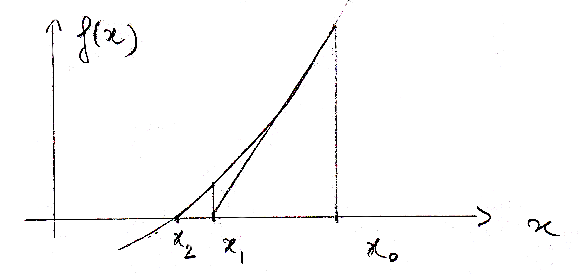
\includegraphics[scale=0.5]{newton-dim1.png}
    \end{figure}

    Nous sommes dans le cadre de la méthode des approximations successives :
    on cherche une solution de $\Phi(x) = x$ avec $\Phi(x) = x - Df(x)^{-1}f(x)$.
    La méthode itérative (\ref{eq:newton}) s'écrit $x_{k+1} = \Phi(x_k)$.


    \begin{ftheo}
        Soit $f : \R^n \longrightarrow \R^n$ de classe $\mathcal{C}^2$ au voisinage de $a \in \R^n$, avec $f(a) = 0$.
        On suppose que $Df(a)$ est inversible. Alors la fonction $\Phi$ de l'itération
        (\ref{eq:newton}) est $\mathcal{C}^1$ au voisinage de $a$, et $a$ est asymptotiquement
        stable. De plus, il existe $\eta > 0$ et $\alpha > 0$ tels que si
        $\norm{x_0 - a} < \eta$ alors :
        \[
            \norm{x_{k+1} - a} \leq \alpha \norm{x_k - a}^2 \hspace{0.5cm} \forall k \geq 0
        \]
    \end{ftheo}

    \begin{remark}
        On dit qu ela convergence de la méthode de Newton est en moyenne \underline{quadratique}.
        On obtient par récurrence :
        \[
            \norm{x_k - a} \leq \frac{1}{\alpha}(\alpha \norm{x_0 - a}^{2^k}
        \]
        Par exemple, si $\alpha = 1$ et $\norm{x_0 - a} = 10^{-1}$, $\norm{x_4 - a} \leq 10^{-16}$.
    \end{remark}

    \begin{preuve}
        La fonction $x \longmapsto \Det Df(x)$ est continue sur $\R^n$, et $\Det Df(a) \ne 0$,
        donc $\exists r > 0 \; / \; \norm{x-a} < r \implies \Det Df(x) \ne 0$,
        c'est-à-dire que $Df(x)$ est inversible. La fonction $\Phi$ définie par
        $\Phi(x) = x - Df(x)^{-1} f(x)$ est donc $\mathcal{C}^1$ au voisinage de $x=a$.
        On peut donc appliquer le théorème 1.

        Calculons $D\Phi(a)$.
        \begin{align*}
            f(a+h) & = Df(a)h + \mathcal{O}(\norm{h}^2) \hspace{0.5cm} \text{ amène :} \\[6pt]
            \Phi(a+h) & = a + h - Df(a+h)^{-1} \Big(Df(a)h + \mathcal{O}(\norm{h}^2) \Big) \\
            & = a + h - \Big( Df(a) \gO(\norm{h} \Big) \Big( Df(a)h + \gO(\norm{h}^2) \Big) \\
            & = a + h - \Big( I + \gO(\norm{h})^{-1} \Big) Df(a)^{-1} \Big( Df(a)h + \gO(\norm{h}^2) \Big) \\
            & = a + h - \Big( I + \gO(\norm{h} \Big) \Big( h + \gO(\norm{h}^2) \Big) \\
            \Phi(a+h) & = \Phi(a) + \gO(\norm{h}^2)
        \end{align*}

        Donc :
        \[
            D\Phi(a) = 0 \implies \text{$a$ est un point fixe de $\Phi$ asymptotiquement stable}
        \]

        Avec $x_k = a + e_k$ on obtient $e_{k+1} = \Phi(a+e_k) - \Phi(a) = \gO(\norm{e_k}^2)$

    \end{preuve}

    \begin{remark}
        \begin{enumerate}[-]
            \item Lorsque la forme analytique de $Df(x)$ est inconnue, on approche
                $\displaystyle\frac{\partial f_i}{\partial x_j}$ par $\displaystyle\frac{f_i(x_1,\dots,x_{j-1},x_{j+\delta},x_{j+1},\dots,x_n) - f_i(x_1, \dots, x_n)}{\delta}$ avec $\delta \approx 0$.

            \item Comme précédemment, le théorème 2 donne la convergence \underline{locale}
                de la méthode de Newton, i.e. pour une condition suffisamment proche d'un
                point fixe $a$.

            \item Avantage de Newton : convergence très rapide (quadratique).

            \item Inconvénient de Newton : coût très élevé à chaque étape, car il faut
                calculer à chaque fois $A_k = Df(x_k)$ et résoudre un système linéaire
                $A_k(x_{k+1} - x_k) = -f(x_k)$ (coût en $\gO(n^3)$, cf méthode de Gauss).
        \end{enumerate}

        $\implies$ plusieurs modifications de la méthode ont été proposées. Nous verrons
        par exemple en TD la méthode de \underline{Broyden} très employée.
        
        Voici une autre modification (plus simple mais efficace) de Newton :
        \begin{equation*}
            \left\lbrace
            \begin{split}
                x_{k+1}  = \Phi(x_k) & \hspace{1cm} & \Phi(x_k) = x_k - A^{-1}f(x_k) \\
                x_0  \in \R^n & & A = Df(x_0)
            \end{split}
            \right.
        \end{equation*}

        On calcule une seule fois la factorisation LU de la matrice $A$, et on l'utilise
        à chaque étape pour résoudre $A(x_{k+1} - x_k) = -f(x_k)$ (coût $\gO(n^2)$ pour $k\geq 2$).

        L'inconvénient est bien sûr qu'on \underline{perd la convergence quadratique} pour
        une convergence uniquement \underline{linéaire}. En effet, si $f(a) = 0$,
        $D\Phi(a) = I - A^{-1}Df(a) \approx 0$ si $x_0 \approx a$, mais
        $\rho \Big( D\Phi(a) \Big) \ne 0$ en général.

        Ce schéma se généralise en remplaçant $A$ par $Df(x_k)$ toutes les ``quelques
        itérations''.
    \end{remark}

\end{document}




